\documentclass[a4paper,11pt,hidelinks]{scrartcl}

\usepackage[ngerman]{babel}
\usepackage{graphicx}
\usepackage{url}
\usepackage{hyperref}
\usepackage{listings}
\usepackage{fontspec}
    \setmainfont{Vollkorn}
    \setsansfont{Lato}
    \setmonofont{Inconsolata}

\renewcommand{\baselinestretch}{1.25}
\pagestyle{headings}

\newcommand{\imgref}[1]{{Abbildung \ref{#1}, Seite \pageref{#1}}}
\lstset{basicstyle=\ttfamily}

\begin{document}

\author{Patrick Bucher}
\title{v13r g3w1nn7}
\subtitle{Gamedesign-Portfolio: Vier gewinnt für Sysadmins}
\date{\today}
\maketitle
\thispagestyle{empty}

\begin{center}
    %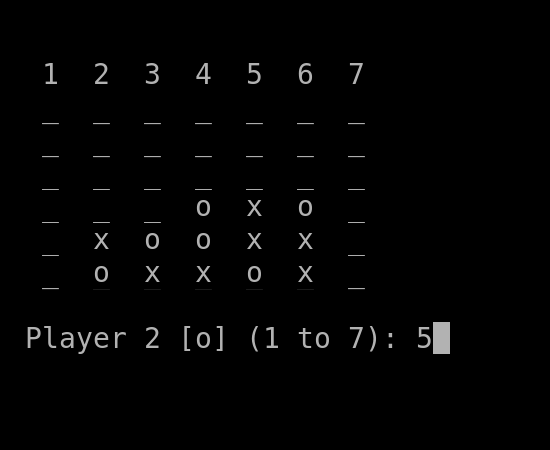
\includegraphics[width=0.5\linewidth]{pics/title.png}
    \begin{lstlisting}
        1 2 3 4 5 6 7                     1 2 3 4 5 6 7
        _ _ _ _ _ _ _                     _ _ _ _ _ _ _
        _ _ _ _ _ _ _                     _ _ _ _ _ _ _
        _ _ _ _ _ _ _                     _ _ _ _ O _ _
        _ _ _ o x o _                     _ _ _ O x o _
        _ x o o x x _                     _ x O o x x _
        _ o x x o x _                     _ O x x o x _

  Player 2 [o] (1 to 7): 5          Player 2 has won the game.
    \end{lstlisting}
\end{center}

\section*{Abstract}

«Vier gewinnt» ist ein weit verbreitetes und bekanntes Strategiespiel für zwei Personen, bei der es darum geht, vier Spielsteine auf einem 7x6-Raster in eine horizontale, vertikele oder diagonale Reihe zu bringen. Zu Zeiten der Corona-Krise lässt sich das Spiel schlecht in physischer Gegenwart an einem Tisch spielen. Ausserdem schaffen die altbekannten Spielregeln und -mechaniken kaum noch einen Anreiz für das Spiel. In der vorliegenden Arbeit soll das Spiel «Vier gewinnt» mit neuen Mechaniken interessanter und besonders auf die Personengruppe der Systemadministratoren angepasst werden, die das Spiel lieber auf der Kommandozeile als in der physichen Version spielen.

\newpage

\tableofcontents
\newpage

\section{Erste Iteration: Zieldefinition und Konzept}

Systemadministratoren (kurz: Sysadmins) haben es nicht einfach zu Zeiten der Corona-Krise: Ins Home-Office verbannt sind sie teilweise ihrer letzten sozialen Kontakte beraubt, zumal \textit{Star Wars}-Conventions und andere Veranstaltungen für Nerds alle abgesagt worden sind ‒ und dies auf eine lange Zeit hinaus. Als kleinen Trost sollen sie ein kleines Computerspiel bekommen, das im Rahmen dieses Projekts konzipiert und entwickelt wird. Dabei handelt es sich um eine erweiterte Version des Spiels «Vier gewinnt» (siehe \imgref{fig:vier-gewinnt}).

Sysadmins haben spezielle Bedürfnisse.\footnote{Als Sysadmins werden im Rahmen der vorliegenden Arbeit nur die Mitglieder der höchsten Kaste bezeichnet ‒ die Unix-Systemadministratoren. Auf die Bedürfnisse der Angehörigen tieferer Kasten soll hier nicht eingegangen werden.} Das herkömmliche «Vier gewinnt» ist ihnen zu langweilig, zumal sie sämtliche Speilverläufe schon längst nachtsüber auf einem ihrer High-End-Server durchgerechnet haben. Zudem ist ihnen nach Spielende das lästige Sortieren der Steine nach Farben, das beim «Vier gewinnt» im Meatspace nötig ist, ein Graus, zumal Sysadmins solche mechanischen Abläufe lieber automatisieren. Ausserdem lassen sich die Spielverläufe beim physischen Spiel nur sehr umständlich und schlecht maschinenlesbar festhalten, etwa mittels Fotokamera.

\begin{figure}
    \centering
    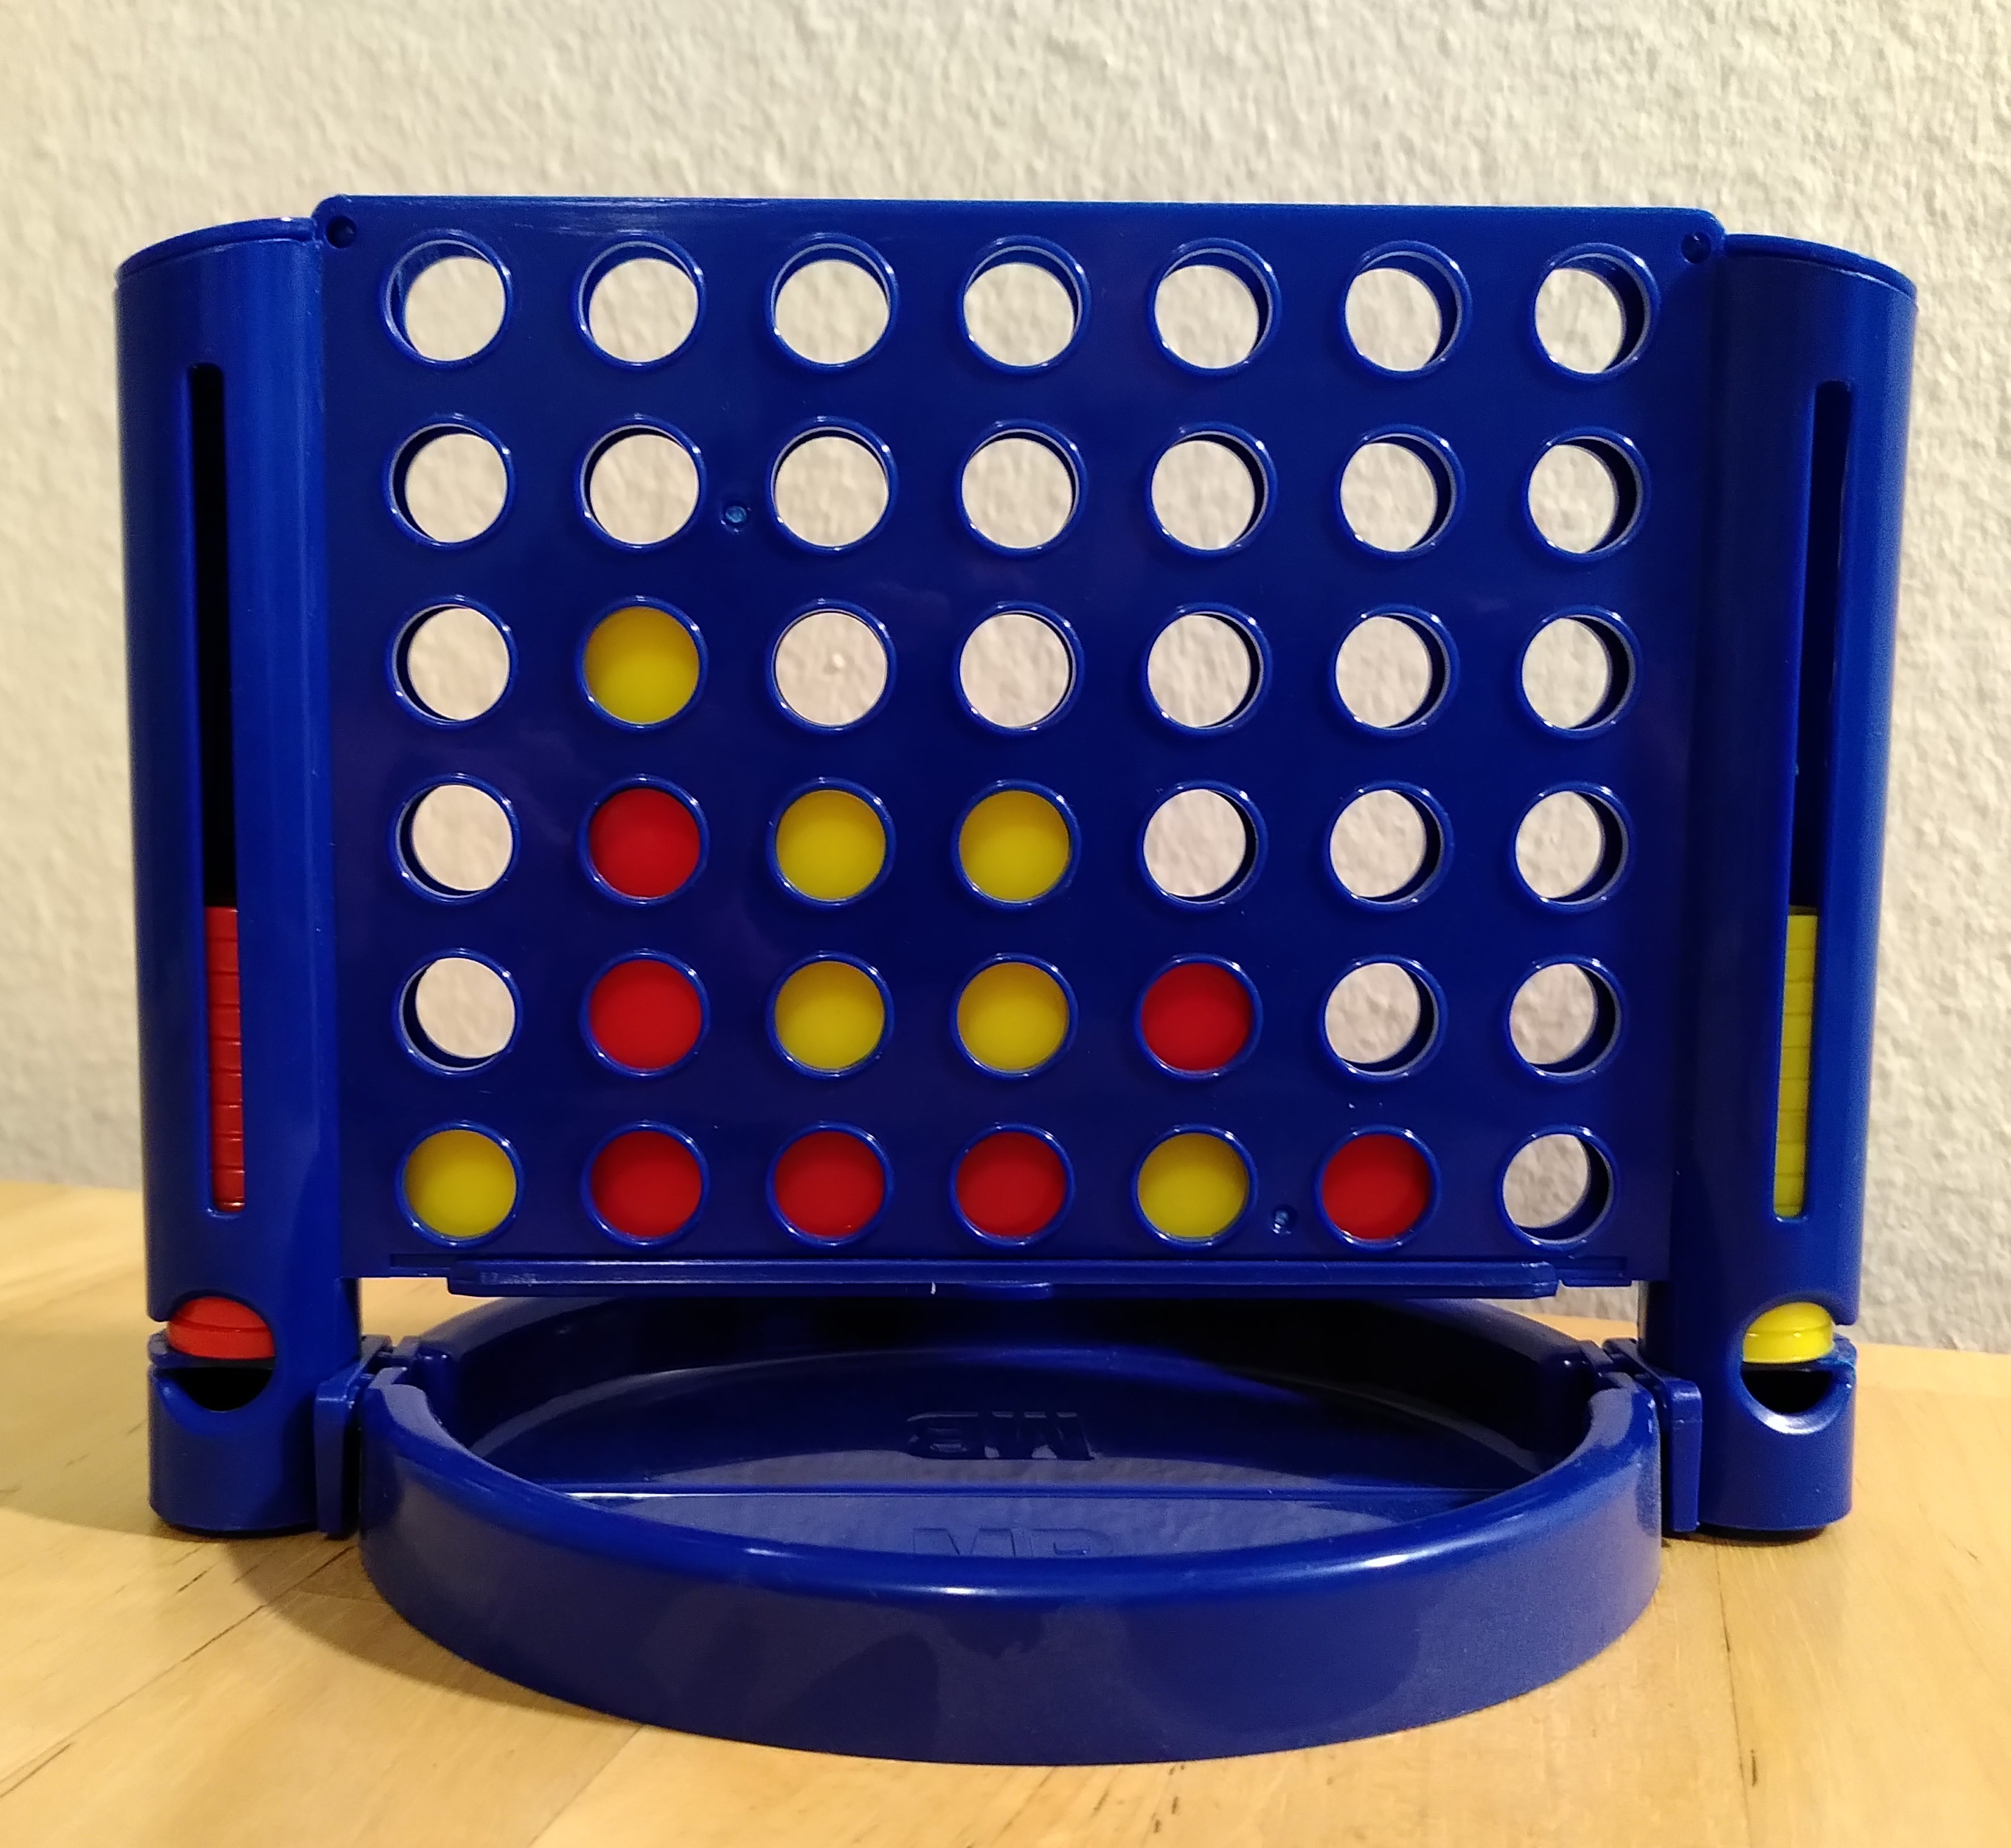
\includegraphics[width=1.0\linewidth]{pics/vier-gewinnt.jpg}
    \caption{Das klassische «Vier gewinnt» (Meatspace-Version). Die grellen Farben der VGA-Palette überfordern das auf die monochrome Bildschirmdarstellung optimierte Auge eines Sysadmins. Das analoge Einwerfen der Steine in die Schächte weckt traumatische Erinnerungen an die Handhabung einer Computermaus.}
    \label{fig:vier-gewinnt}
\end{figure}

\subsection{Vorteile der Kommandozeilenversion}

«Vier gewinnt» wäre viel besser, wenn man es auf der Kommandozeile spielen könnte! Dies hätte folgende Vorteile gegenüber der herkömmlichen Meatspace-Version:

\begin{enumerate}
    \item Das Spiel könnte während der Arbeitszeit gespielt werden, ohne dass der gelegentlich vorbei- und in den Bildschirm schauende Vorgesetzte diese Strategie der Arbeitsvermeidung als solche erkennen könnte. Schliesslich handelt es sich ja bloss um irgendwelche kryptisch anmutende Zeichen, die da auf dem Bildschirm zu sehen sind. Bestimmt hat der Sysadmin da einen Belegungsplan für Pins oder dergleichen auf dem Bildschirm, und selbstverständlich handelt es sich dabei um geistige Schwerstarbeit, die dem Arbeitgeber zugute kommt ‒ das verrät schon des Sysadmins angestrengter Gesichtsausdruck!
    \item Die Aufforderung der Geschäftsleitung, mehr zu kommunizieren und sich Probleme gemeinsam anzuschauen, könnte für weitere Arbeitsvermeidung ausgenutzt werden, indem sich zwei Sysadmins am gleichen Computer treffen, um dort «Vier gewinnt» (bzw. \texttt{v13r g3w1nnt!!!11}) zu spielen. Die kryptisch anmutende Pin-Be\-le\-gung, die da für den Vorgesetzten auf dem Bildschirm zu sehen ist, schreit ja geradezu nach einer \textit{Pair Debugging Session}! So kann die Arbeitszeit weiter mit «Vier gewinnt» vertrödelt werden, und die sozialen Kontakte der Firma werden dadurch noch weiter gestärkt ‒ ganz im Sinne der Geschäftsleitung!
    \item Da solche sozialen Interaktionen im Meatspace derzeit wegen \textit{Social Distancing} kaum denkbar sind, müsste das Spiel auch remote von zwei Sysadmins spielbar sein, ohne dass die Nerds der Softwareentwicklung das Spiel aufwändig umprogrammieren müssen. So könnten die Sysadmins das Spiel von zu Hause aus über eine gemeinsame Session mit \texttt{tmux} oder GNU \texttt{screen} gegeneinander spielen. Dies dürfte auch die VPN-Verbindung ins Büro nicht weiter beeinträchtigen, zumal diese schon durch BitTorrent-Downloads voll ausgelastet ist. Der Multiplayer-Modus wäre somit auch über eine serielle Verbindung möglich, die der erfahrene Sysadmin notfalls auch aus im Büro gestohlenen Büroklammern und aus abgerissenen Streifen seines Aluhuts herstellen könnte. Sollte der Bildschirm des Sysadmins unerwartet in die Brüche gehen, wäre das Spiel immer noch über einen Fernschreiber spielbar, der sich bei jedem guten Systemadmin im Keller finden lässt.\footnote{In der Regel hinter der Kiste mit den \textit{Star Trek}-Fanartikeln.}
    \item Die Spielverläufe können einfach in Textdateien\footnote{d.h. MIME-Type \texttt{text/html;charset=utf-8}, selbstverständlich ohne \textit{byte order mark} (BOM)} festgehalten werden. Das erleichtert die Diskussion über Spielstrategien auf dem Usenet und in IRC.
\end{enumerate}

Das klassische «Vier gewinnt» müsste hierzu natürlich noch etwas interessanter ausgestaltet werden, sodass die Motivation der Sysadmins zumindest das Warten auf den nächsten Download auf den derzeit chronisch überlasteten Steam-Servern überdauert. Diese möglichen Verbesserungen sollen im Rahmen dieser Arbeit vorgeschlagen, umgesetzt und evaluiert werden.

\subsection{Zwei Tastaturen, eine Kommandozeile}

Um das Treffen zweier Sysadmins auf einem gemeinsamen Terminal, das für die Evaluation des Prototyps nötig ist, zu bewerkstelligen, muss ein gemeinsam zugänglicher Server zuerst entsprechend konfiguriert werden.\footnote{Server können von HSLU-Studierenden kostenlos und unkompliziert im \textit{Enterprise Lab} bezogen werden. Diese dürften knapp genügend Leistung aufbringen, um eine Anbindung mit einer Baudrate von 9600 über längere Zeit zu gewährleisten. Mit neueren Versionen von Solaris dürfte sich auch \texttt{tmux} einfach installieren lassen (siehe \url{https://www.opencsw.org/packages/tmux/}).}

Sollte wider aller Erwartung kein Solaris, sondern ein Debian-basiertes Betriebssystem auf dem Server installiert sein, lässt sich die gemeinsame Spielumgebung mit den folgenden Schritten einrichten.

Zunächst muss \texttt{tmux} installiert werden:

\begin{lstlisting}
# apt-get install tmux
\end{lstlisting}

Als nächstes ist eine gemeinsame Benutzergruppe und je ein Benutzer für die beiden Spieler (\texttt{geek} und \texttt{poke}) zu erstellen. Auch müssen den neu erstellen Benutzern gleich Passwörter hinterlegt werden:

\begin{lstlisting}
# groupadd sysadmins
# useradd -G sysadmins -m geek
# useradd -G sysadmins -m poke
# passwd geek
# passwd poke
\end{lstlisting}

Das \texttt{\$HOME}-Verzeichnis, das über das \texttt{-m}-Flag erstellt wird, ist wichtig, da die beiden Spieler ihre Spielverläufe ja schliesslich in Textdateien festhalten und kommentieren wollen ‒ letzteres vorzugsweise mit \texttt{ed(1)}, dem Standard-Texteditor von Unix.

Nun kann sich der erste Benutzer (\texttt{geek}) auf dem Server einloggen und eine neue \texttt{tmux}-Session namens \texttt{game} eröffnen:

\begin{lstlisting}
[geek]$ tmux -S /tmp/shared new -s game
\end{lstlisting}

Die Session muss so berechtigt werden, dass alle Benutzer der Gruppe \texttt{sysadmins} darauf zugreifen können:

\begin{lstlisting}
[geek]$ chgrp sysadmins /tmp/shared
\end{lstlisting}

Anschliessend kann sich der zweite Benutzer (\texttt{poke}) einloggen und an der bestehenden \texttt{tmux}-Session teilnehmen:

\begin{lstlisting}
[poke]$ tmux -S /tmp/shared attach -t game
\end{lstlisting}

Jetzt benötigen die beiden Spieler bloss noch ein Spiel, und der Spass kann auf einer tiefen Bandbreite beginnen!

\subsection{Prototyp für «Vier gewinnt»}

In dieser ersten Iteration soll nur das herkömmliche «Vier gewinnt»-Spiel zum Einsatz kommen. Dieses wird zunächst in einer Kommandozeilenversion entwickelt.

Als Umsetzungsplattform für den Prototyp kommt Python 3 zum Einsatz. Mit dieser Programmiersprache hat der Autor dieser Arbeit bereits einiges an positiver Erfahrung sammeln können. Ausserdem verfügt Python mit NumPy\footnote{\url{https://numpy.org/}} über eine mächtige Library für (mehrdimensionale) Arrays, mit der sich viele Listenoperationen mit wenig Code und effizient umsetzen lassen.\footnote{Für die richtige Version des Spiels würde eine Programmiersprache verwendet werden, die eine höhere Laufzeitperformance bei geringerem Speicherverbrauch ermöglicht, wie z.B. ANSI C 89, Assembler oder Fortran 66, damit der Sysadmin sich nicht unnötig Rechenpower für das Bitcoin-Mining verliert.}

Die Spiellogik wird mithilfe von pytest\footnote{\url{https://docs.pytest.org/en/latest/}} automatisiert getestet. Auch wenn es sich nur um einen Prototyp handelt, ist die Korrektheit der Spiellogik ein wichtiger Usability-Faktor, zumal nicht erkannte Gewinnsituationen für die Beteiligten sehr frustrierend sind, was einen negativen Einfluss auf die Testläufe hätte.

Der Prototyp ist einfach zu bedienen und schliesst Fehleingaben so gut wie möglich aus. Das Folgende Kommandozeilenfenster zeigt den Prototyp während eines Spiels:

\begin{lstlisting}
        1 2 3 4 5 6 7
        _ _ _ _ _ _ _
        _ _ _ _ _ _ _
        _ _ _ _ _ _ _
        _ x _ _ o _ _
        _ o x o o o x
        _ x o x x x o

Player 1 [x] (1 to 7): ¶
\end{lstlisting}

Das Spielfeld wird mit einem 7x6-Raster dargestellt. Der Underscore (\texttt{\_}) markiert dabei leere Felder. Spieler 1 spielt mit dem Spielstein \texttt{x}, und Spieler 2 mit dem Spielstein \texttt{o}. Die Titelzeile markiert die einzelnen Spalten (oder «Schächte») mit einer Nummer, sodass sich der Spieler beim Auswählen des Schachts einfacher orientieren kann.

Das Paragraph-Zeichen (\texttt{¶}) markiert die Eingabeaufforderung. Der Spieler soll die Nummer des Schachts auswählen, in den sein Spielstein fallen soll. Falscheingaben (nicht numerische, nicht im Bereich 1-7, einen vollen Schacht bezeichnend usw.) werden nicht akzeptiert, sondern mit einer Fehlermeldung und einer erneuten Eingabeaufforderung quittiert:

\begin{lstlisting}
        1 2 3 4 5 6 7
        _ _ _ _ x _ _
        _ _ _ _ o _ _
        _ _ _ _ x _ _
        _ x _ _ o _ _
        _ o x o o o x
        _ x o x x x o

Player 2 [o] (1 to 7): 5
You must pick a free slot between 1 and 7!
\end{lstlisting}

Sind alle Spielfelder voll, ohne dass dabei ein Spieler die Siegbedingung (vier Spielsteine in einer horizontalen, vertikalen oder diagonalen Reihe) erfüllt, wird das Spiel als unentschieden gewertet. Erfüllt ein Spieler die Siegbedingung, ist das Spiel zu Ende und der Sieger wird als solcher ausgewiesen:

\begin{lstlisting}
        1 2 3 4 5 6 7
        _ _ _ _ x _ _
        _ _ _ _ o _ _
        _ _ _ _ X _ _
        _ x _ X o o _
        _ o X o o o x
        _ X o x x x o

Player 1 has won the game.
\end{lstlisting}

Hierbei wird zur leichteren Erkennung die Siegreihe hervorgehoben, indem der Spielstein durch einen entsprechenden Grossbuchstaben ersetzt wird (\texttt{x} wird hier durch \texttt{X} ersetzt). Dies soll Diskussionen zwischen aufbegrachten Sysadmins verhindern, die ansonsten nur in die Richtung gehen würde, dass diese Software halt falsch programmiert worden sei ‒ und die Erkennung der Siegbedingung nicht ausreichend getestet.

Das Spiel ist bereit für die erste Testreihe: Das Testen der Grundversion.

\newpage

\section{Zweite Iteration: Anwendung von Game-Design-Theorie}

\subsection{Entscheidungen}

Verschiedene Spiele lassen verschiedene Arten von Entscheidungen zu. Bei einfachen Spielen hat man es v.a. mit uninteressanten Entscheidungen zu tun. Diese lassen sich in die folgenden Kategorien aufteilen:

\begin{description}
    \item[Keine Entscheidungen] Das Würfeln bei einem Leiterlispiel ist keine Entscheidung, da hier der Zufall regiert. Bei jeder Runde muss gewürfelt werden, der Spieler kann darüber nicht entscheiden.
    \item[Bedeutungslose Entscheidungen] Das Tippen auf Kopf oder Zahl beim Münzwurf ist eine bedeutungslose Entscheidung. Es muss eine Entscheidung getroffen werden, die das Spielergebnis aber nicht beeinflusst, bzw. vom Glück abhängig ist.
    \item[Offensichtliche Entscheidungen] Das setzen eines Steines in «Vier gewinnt» ist eine offensichtliche Entscheidung. Aus der Spielmechanik geht etwa klar hervor, welche Eröffnungszüge sinnvoll sind (in der Mitte spielen), oder welche Züge den Spieler dem Sieg näherbringen (Einreihung von Steinen).
    \item[Blinde Entscheidungen] Das Wählen einer Koordinate beim «Schiffe versenken» läuft zumeist blind ab, da man das Spielfeld des Gegners nicht kennt. Im Verlauf des Spiels erhält man jedoch immer ein besseres Bild vom Spielfeld des Gegners, sodass in manchen Spielsituationen das Versenken von grossen Schiffen zu einer offensichtlichen Entscheidung werden kann.
\end{description}

Beim Spiel «Vier gewinnt» hat man es mit offensichtlichen Entscheidungen zu tun. Umd as Spiel interessanter zu machen, muss es interessante Entscheidungen zulassen.

Interessante Entscheidungen unterscheiden sich von uninteressanten Enscheidungen u.a. dadurch, dass mit ihnen ein gewisses Risiko einhergeht, das sich nicht oder nur begrenzt abschätzen lässt. Oft wirken sich risikoreiche Entscheidungen nicht schon unmittelbar nach der Entscheidung, sondern erst später auf den Spielverlauf aus.

Bei «Vier gewinnt» steht dem Spieler nur eine Art von Auswahl zur Verfügung: Die Wahl des Schachts, in der ein Stein eingeworfen werden soll. Das Spiel kann dann interessanter werden, wenn andere Arten von Entscheidungen angeboten werden. Je nach Spielsituation wäre dann eine andere Art der Entscheidung angebracht.

\subsection{Balancing}

\newpage

\begin{figure}
    \centering
    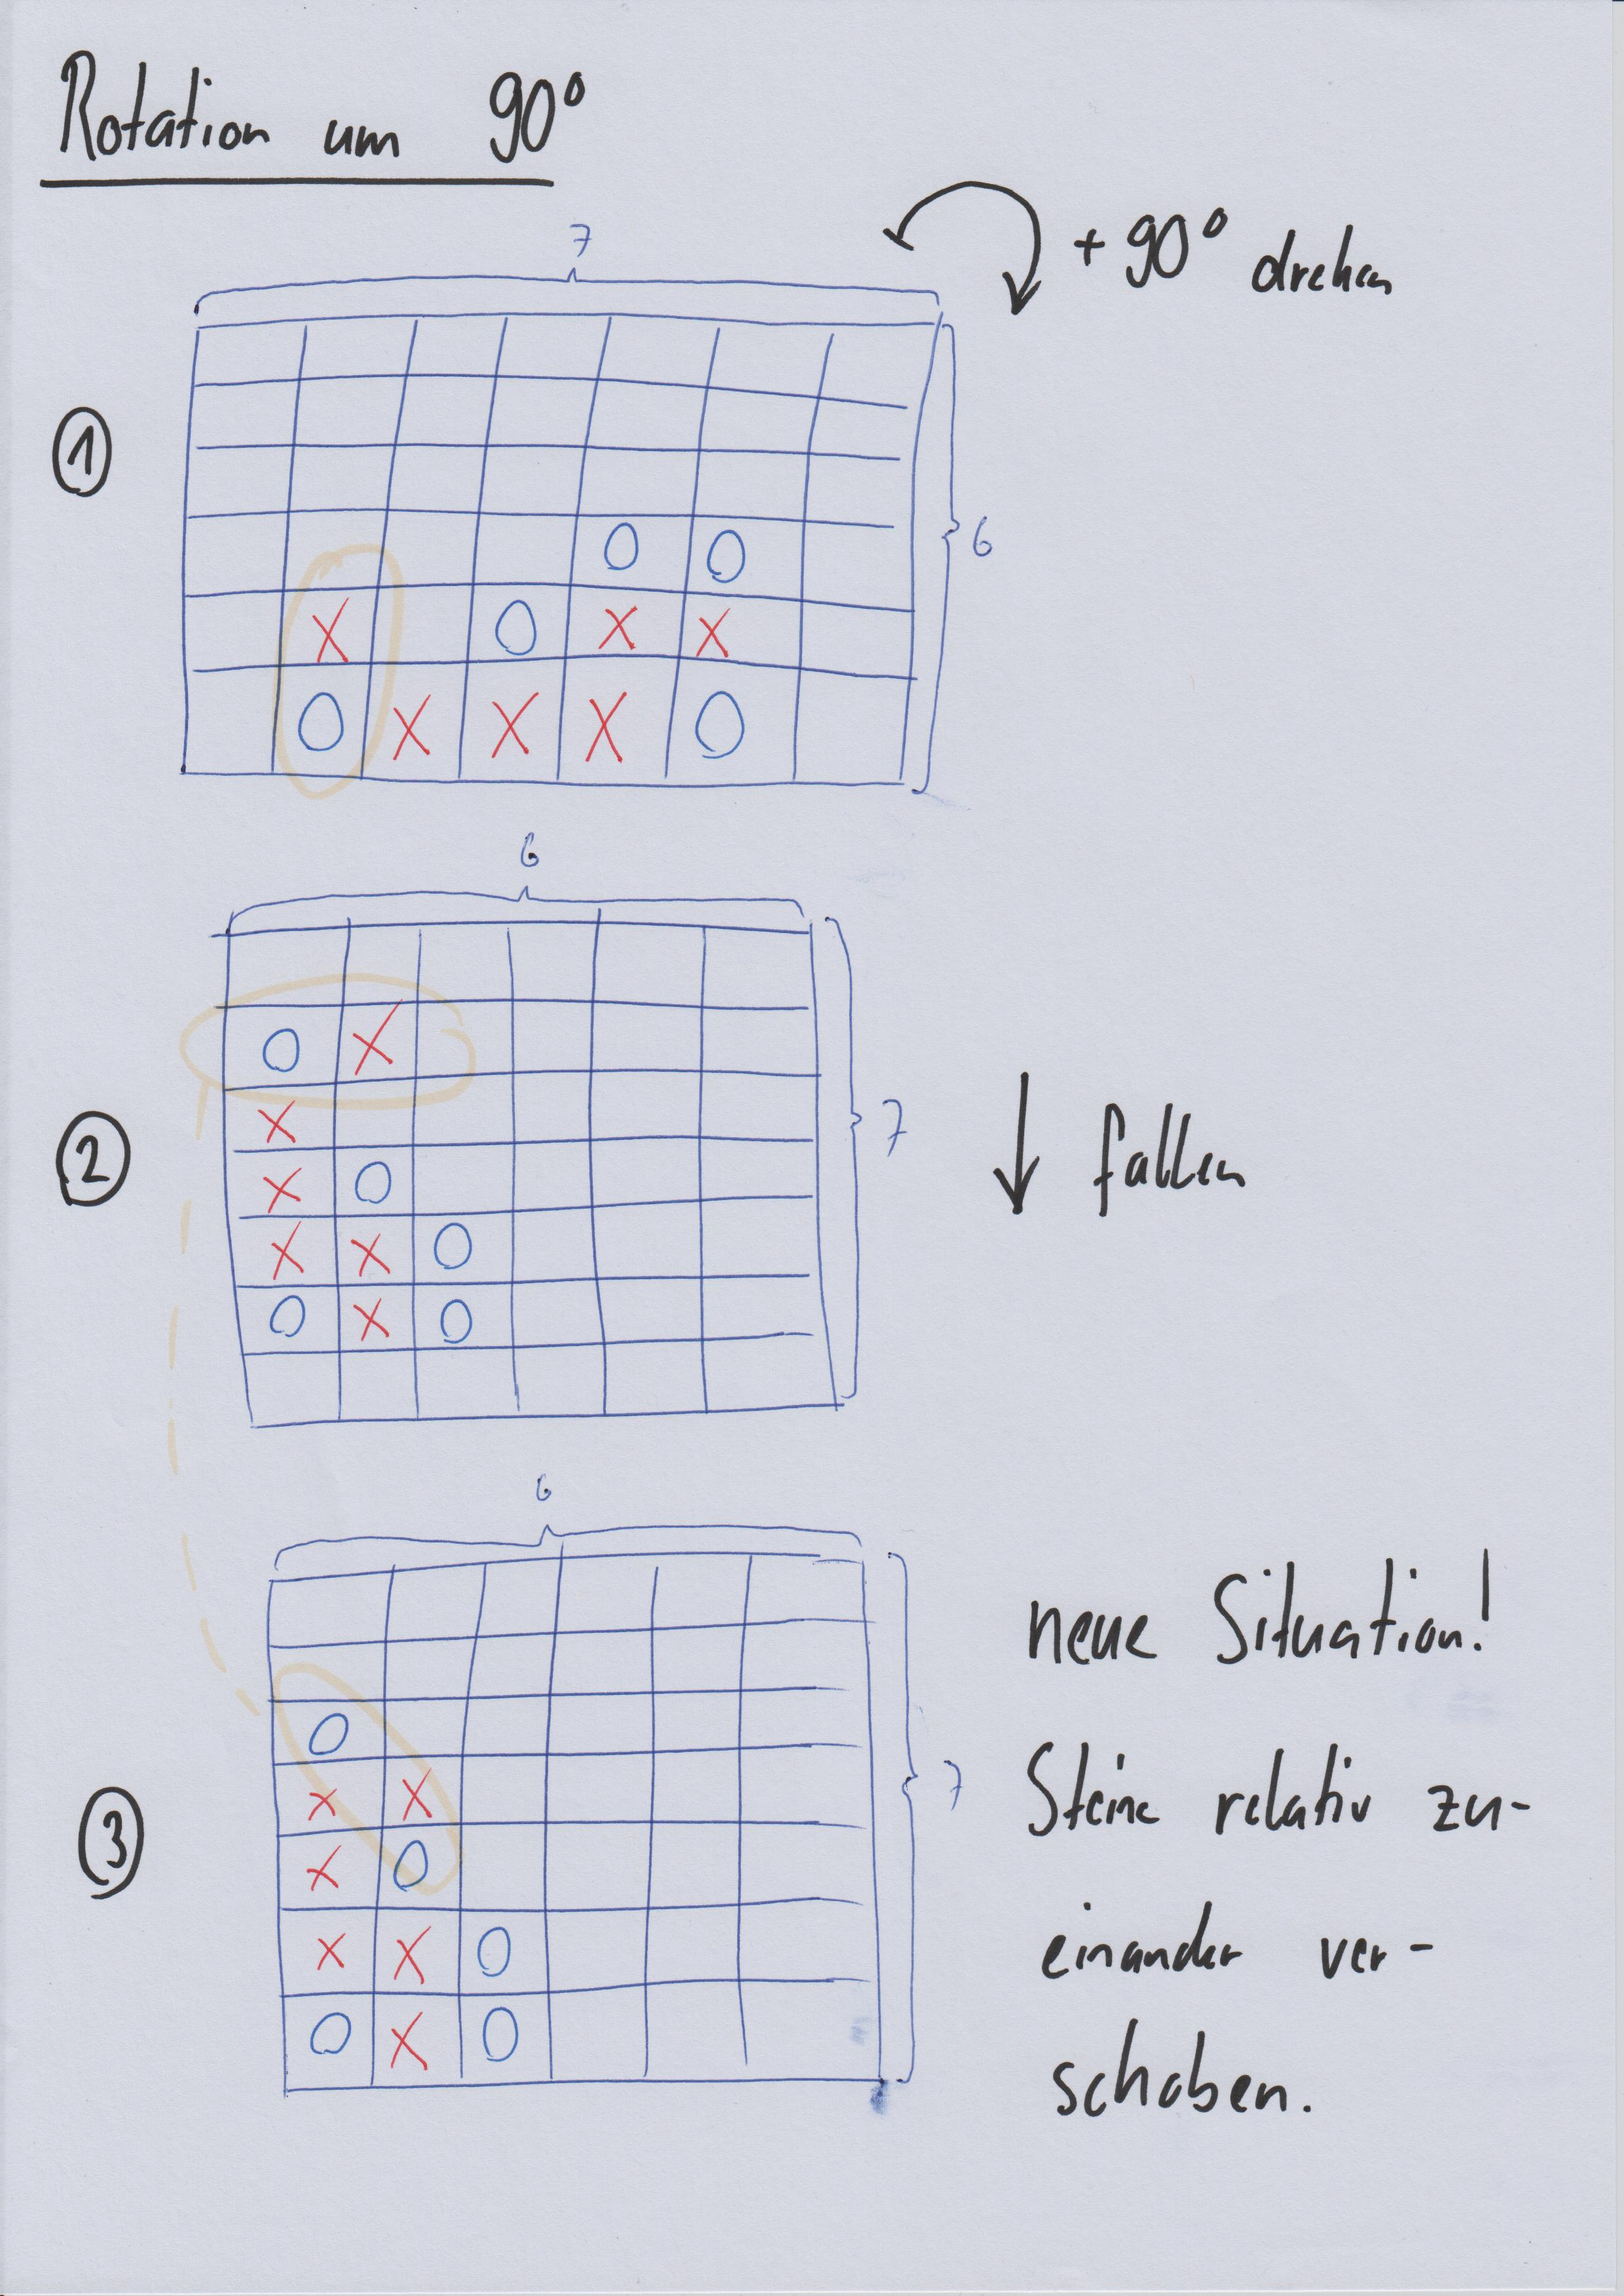
\includegraphics[width=0.8\linewidth]{pics/rotation-papier.jpg}
    \caption{Die Rotation um 90° als zusätzliche Spielmechanik. Das Spielgitter wird zunächst gedreht, anschliessend fallen die Steine nach unten. So entsteht eine neue Spielsituation, da sich manche Steine relativ zueinander bewegen.}
\end{figure}

\section{Dritte Iteration: Abschliessender Nutzertest und Reflexion}
\newpage

\listoffigures
\addcontentsline{toc}{section}{Abbildungsverzeichnis}

\end{document}
